\documentclass[pdf]{beamer}

\usepackage{rsislidepacks}
\usepackage{colortbl}
\usepackage{enumerate}
\usepackage{hyperref}
\usepackage{asymptote}
\usetheme{UNLTheme}
\setbeamercovered{dynamic}

\usepackage{tikz}
\usetikzlibrary{shapes,arrows}

\def\ii{\item}
\def\ul#1{\underline{#1}}

\begin{asydef}
	import olympiad;
	import cse5;
	pointpen = black;
	pathpen = black;
	pathfontpen = black;
	anglepen = black;
	anglefontpen = black;

	pen s = blue, t = red;
	pen dot_s = blue, dot_t = red;
\end{asydef}

\begin{document}
\title[Bott-Samelson Bimodules]{Diagrammatic Computation of Morphisms Between Bott-Samelson Bimodules via Libedinsky's Light Leaves}
\subtitle[RSI 2013]{Research Science Institute 2013}
\author[Evan Chen]{Evan Chen \\ Under the Direction of Francisco Unda, MIT \\ Project Provided by Ben Elias, MIT\vspace{-2em}}
\date{\today}

\begin{frame}
	\maketitle
\end{frame}

\begin{frame}[fragile]
	\frametitle{Background}
	
	% Define block styles
	\tikzstyle{block} = [rectangle, draw, fill=blue!20, text width=5em, text centered, rounded corners, minimum height=4em]
	\tikzstyle{cloud} = [draw, ellipse,fill=red!20, node distance=3cm, text width=6em, text centered, minimum height=2em]
	\tikzstyle{line} = [draw, -latex']
    
	\begin{tikzpicture}[node distance = 4.5cm, auto]
		% Place nodes
		\node [cloud] (Hecke) at (0,6) {Hecke algebra};
		\node [block] (Soergel) at (0,3) {Soergel bimodules};
		\node [block] (KL) at (5,3) {Kazhdan-Lusztig};
		\node [block] (BS) at (0,0) {Bott-Samelson bimodule};
		\node [cloud] (leaf) at (5,0) {Libedinsky's light leaves};
		% Draw edges
		\path [line] (Hecke) -- node [near end] {categorified by} (Soergel);
		\path [line] (Hecke) -- node [near start] {categorified by} (KL);
		\path [line] (Soergel) -- node {described by} (BS);
		\path [line] (leaf) -- node [text width=5em] {constructs morphisms} (BS);
	\end{tikzpicture}
\end{frame}

\begin{frame}[fragile]
	\frametitle{Diagrammatics}
	The maps (morphisms) between Bott-Samelson bimodules can be represented by \alert{diagrams}.
	\begin{figure}[ht]
		\centering
		\begin{asy}
		size(4cm);
		real xmax=7;
		real ymax=5;
		draw( (xmax,ymax)--(xmax,-ymax)--(-xmax,-ymax)--(-xmax,ymax)--cycle );
		pair apex = (0,2);
		path arc = (5,-5)..(2,0)..apex..(-2,0)..(-5,-5);
		draw(arc, s);
		dot(apex, dot_s);
		draw(apex--(0,ymax), s);
		draw(-apex--(0,-ymax), t);
		dot(-apex, dot_t);
		label("$s$", (0,ymax), dir(90));
		label("$t$", (0,-ymax), dir(270));
		label("$s$", (-5,-ymax), dir(270));
		label("$s$", (5,-ymax), dir(270));
		\end{asy}
		\caption{An example of a possible diagram.}
		\label{fig:example_diagram}
	\end{figure}
\end{frame}

\begin{frame}
	\frametitle{Libedinsky's Light Leaves}
	\begin{itemize}
		\ii Expression $\ul r$ with letters $s$ and $t$.
		\ii Binary string $\ul b$.
	\end{itemize}
	\begin{figure}
		\centering
		\only<1>{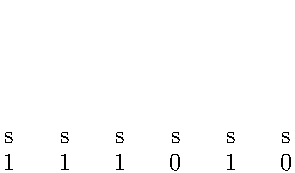
\includegraphics{anime/onecolor_example-1.pdf}}%
		\only<2>{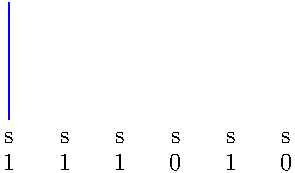
\includegraphics{anime/onecolor_example-2.pdf}}%
		\only<3>{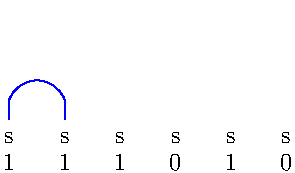
\includegraphics{anime/onecolor_example-3.pdf}}%
		\only<4>{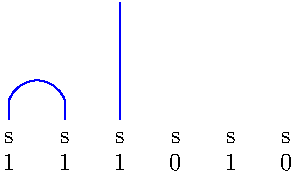
\includegraphics{anime/onecolor_example-4.pdf}}%
		\only<5>{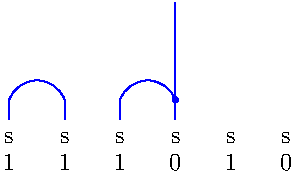
\includegraphics{anime/onecolor_example-5.pdf}}%
		\only<6>{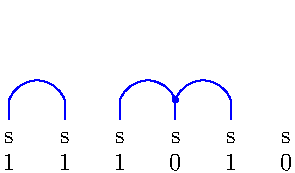
\includegraphics{anime/onecolor_example-6.pdf}}%
		\only<7>{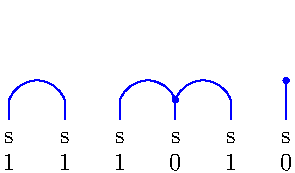
\includegraphics{anime/onecolor_example-7.pdf}}%
		\only<8>{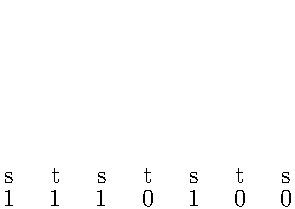
\includegraphics{anime/twocolor_example-1.pdf}}%
		\only<9>{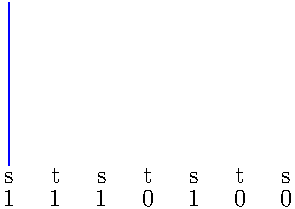
\includegraphics{anime/twocolor_example-2.pdf}}%
		\only<10>{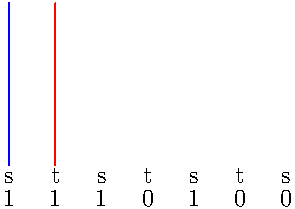
\includegraphics{anime/twocolor_example-3.pdf}}%
		\only<11>{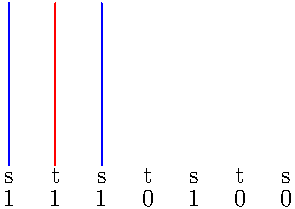
\includegraphics{anime/twocolor_example-4.pdf}}%
		\only<12>{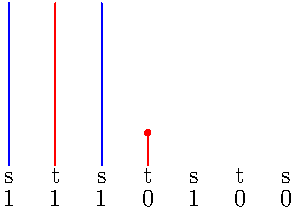
\includegraphics{anime/twocolor_example-5.pdf}}%
		\only<13>{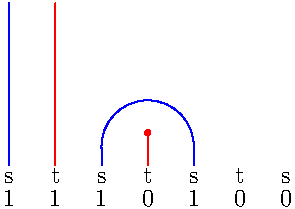
\includegraphics{anime/twocolor_example-6.pdf}}%
		\only<14>{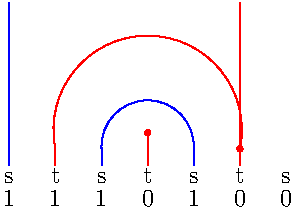
\includegraphics{anime/twocolor_example-7.pdf}}%
		\only<15>{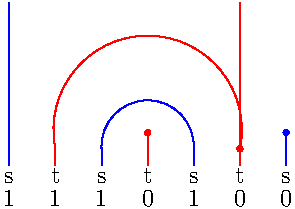
\includegraphics{anime/twocolor_example-8.pdf}}%
	\end{figure}
\end{frame}

\begin{frame}[fragile]
	\frametitle{Composition and Problem Statement}
	\begin{figure}[ht]
		\centering
		\only<1>{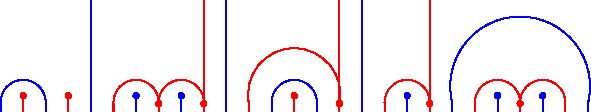
\includegraphics{anime/compose_example-1.pdf}}%
		\only<2>{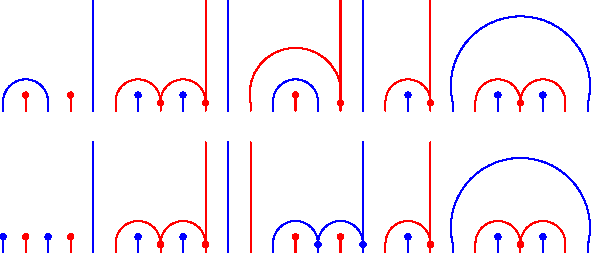
\includegraphics{anime/compose_example-2.pdf}}%
		\only<3-4>{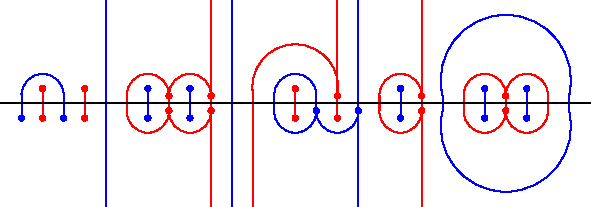
\includegraphics{anime/compose_example-3.pdf}}%
	\end{figure}
	\visible<4>{\alert{Goal}: compute new map based on the binary strings $\ul b_1$, $\ul b_2$, and string $\ul r$.}
\end{frame}


\begin{frame}
	\frametitle{Results}
	\begin{enumerate}
		\ii $\ul r = \underbrace{s\dots s}_{\text{$n$ $s$'s}}$. \pause $\checkmark$ \pause
		\ii $\ul r = \underbrace{stst\dots}_{\text{$n$ characters}}$.
	\end{enumerate}
\end{frame}


\begin{frame}[fragile]
	\frametitle{Definitions}
%	\begin{definition}
%		\begin{itemize}
%			\ii \emph{Barbell}: acyclic component.
%			\ii \emph{Bubble}: bounded face.
%			\ii \emph{Caterpillar}: connected collection of bubbles.
%			\ii \emph{Fence}: dividing line.
%			\ii \emph{Pasture}: regions delimited by fences.
%		\end{itemize}
%	\end{definition}

	\begin{figure}[ht]
		\centering
		\begin{asy}
			size(10cm);
			real h = 0.7;
			int n = 16;

			picture one;
			draw(one, (0,0)--(0,h/2)..((0+2)/2.0,h*2)..(2,h/2)--(2,0), s);
			draw(one, (3,0)--(3,h/2)..((3+6)/2.0,h*3)..(6,h/2)--(6,0), s);
			draw(one, (9,0)--(9,h/2)..((9+11)/2.0,h*2)..(11,h/2)--(11,0), t);
			draw(one, (11,0)--(11,h/2)..((11+13)/2.0,h*2)..(13,h/2)--(13,0), t);
			draw(one, (13,0)--(13,h/2)..((13+15)/2.0,h*2)..(15,h/2)--(15,0), t);
			draw(one, (1,0)--(1,h), t);
			dot(one, (1,h), dot_t);
			draw(one, (4,0)--(4,h), t);
			dot(one, (4,h), dot_t);
			draw(one, (5,0)--(5,h), t);
			dot(one, (5,h), dot_t);
			draw(one, (10,0)--(10,h), s);
			dot(one, (10,h), dot_s);
			draw(one, (12,0)--(12,h), s);
			dot(one, (12,h), dot_s);
			draw(one, (14,0)--(14,h), s);
			dot(one, (14,h), dot_s);
			draw(one,(7,0)--(7,4*h), t);
			draw(one,(8,0)--(8,4*h), s);
			dot(one, (11, h/2), dot_t);
			dot(one, (13, h/2), dot_t);

			picture two;
			draw(two, (3,0)--(3,h/2)..((3+6)/2.0,h*3)..(6,h/2)--(6,0), s);
			draw(two, (9,0)--(9,h/2)..((9+11)/2.0,h*2)..(11,h/2)--(11,0), t);
			draw(two, (11,0)--(11,h/2)..((11+13)/2.0,h*2)..(13,h/2)--(13,0), t);
			draw(two, (13,0)--(13,h/2)..((13+15)/2.0,h*2)..(15,h/2)--(15,0), t);
			draw(two, (0,0)--(0,h), s);
			dot(two, (0,h), dot_s);
			draw(two, (1,0)--(1,h), t);
			dot(two, (1,h), dot_t);
			draw(two, (2,0)--(2,h), s);
			dot(two, (2,h), dot_s);
			draw(two, (4,0)--(4,h), t);
			dot(two, (4,h), dot_t);
			draw(two, (5,0)--(5,h), t);
			dot(two, (5,h), dot_t);
			draw(two, (10,0)--(10,h), s);
			dot(two, (10,h), dot_s);
			draw(two, (12,0)--(12,h), s);
			dot(two, (12,h), dot_s);
			draw(two, (14,0)--(14,h), s);
			dot(two, (14,h), dot_s);
			draw(two,(7,0)--(7,4*h), t);
			draw(two,(8,0)--(8,4*h), s);
			dot(two, (11, h/2), dot_t);
			dot(two, (13, h/2), dot_t);

			add(one); add(reflect((0,0),(1,0))*two);
			draw((-1,0)--(16,0));

			label("Pastures", (7.5,6*h));
			draw((7,5.5*h)--(4,4*h), EndArrow);
			draw((7.5,5.5*h)--(7.5,4*h), EndArrow);
			draw((8,5.5*h)--(11,4*h), EndArrow);
			label("Bubble", (4.5,-3*h), dir(-90));
			label("Fences", (7.5,-4*h), dir(-90));
			label("Barbells", (1, 4*h));
			draw((1,3.5*h)--(1,2.5*h), EndArrow);
			label("Caterpillar", (12,-2*h), dir(-90));
		\end{asy}
	\end{figure}
\end{frame}

\begin{frame}[fragile]
	\frametitle{Bubble Lemma}
	\begin{lemma}[Bubble Lemma]
		If $\ul r = stst\dots$, then
		every bubble contains either a single caterpillar or a single barbell.
	\end{lemma}
	\begin{figure}[ht]
		\centering
		\begin{asy}
		size(3cm);
		real h = 0.7;
		int n = 7;

		picture one;
		draw(one, (1,0)--(1,h/2)..((1+3)/2.0,h*2)..(3,h/2)--(3,0), t);
		draw(one, (3,0)--(3,h/2)..((3+5)/2.0,h*2)..(5,h/2)--(5,0), t);
		draw(one, (0,0)--(0,h/2)..((0+6)/2.0,h*6)..(6,h/2)--(6,0), s);
		draw(one, (2,0)--(2,h), s);
		dot(one, (2,h), dot_s);
		draw(one, (4,0)--(4,h), s);
		dot(one, (4,h), dot_s);
		dot(one, (3, h/2), dot_t);

		picture two;
		draw(two, (1,0)--(1,h/2)..((1+3)/2.0,h*2)..(3,h/2)--(3,0), t);
		draw(two, (3,0)--(3,h/2)..((3+5)/2.0,h*2)..(5,h/2)--(5,0), t);
		draw(two, (0,0)--(0,h/2)..((0+6)/2.0,h*6)..(6,h/2)--(6,0), s);
		draw(two, (2,0)--(2,h), s);
		dot(two, (2,h), dot_s);
		draw(two, (4,0)--(4,h), s);
		dot(two, (4,h), dot_s);
		dot(two, (3, h/2), dot_t);

		add(one); add(reflect((0,0),(1,0))*two);
		draw((-1,0)--(7,0));
		\end{asy}
		\caption{A bubble with a caterpillar inside it}
	\end{figure}
\end{frame}

\begin{frame}
	\frametitle{Other Lemmas}
	\begin{lemma}[Caterpillar Lemma]
		Technical result about the possible values of a caterpillar.
	\end{lemma}
	\pause
	\begin{lemma}[Pasture Lemma]
		Caterpillars appear only in the leftmost and rightmost pastures.
	\end{lemma}
	\pause
	\[ \text{Lemmata} \implies \text{Algebraic Results} \implies \text{:)} \]
\end{frame}

%\begin{frame}[fragile]
%	\frametitle{Pasture Theorem}
%	\begin{theorem}[Pasture Theorem]
%		 If pastures are labelled $0, 1, \dots, N$ then:
%		\begin{itemize}
%			\ii Pastures $1$ through $N-1$ must contain caterpillars attached to fences.
%			\ii Pasture $N$ is either empty or contains a single caterpillar.
%		\end{itemize}
%	\end{theorem}
%	\begin{figure}[ht]
%		\centering
%		\begin{asy}
%			size(3cm);
%			real h = 0.7;
%			int n = 9;
%
%			picture one;
%			draw(one, (2,0)--(2,h/2)..((2+4)/2.0,h*2)..(4,h/2)--(4,0), s);
%			draw(one, (1,0)--(1,h/2)..((1+5)/2.0,h*4)..(5,h/2)--(5,0), t);
%			draw(one, (6,0)--(6,h/2)..((6+8)/2.0,h*2)..(8,h/2)--(8,0), s);
%			draw(one, (3,0)--(3,h), t);
%			dot(one, (3,h), dot_t);
%			draw(one, (7,0)--(7,h), t);
%			dot(one, (7,h), dot_t);
%			draw(one,(0,0)--(0,5*h), s);
%			draw(one,(5,0)--(5,5*h), t);
%			dot(one, (5, h/2), dot_t);
%
%			picture two;
%			draw(two, (2,0)--(2,h/2)..((2+4)/2.0,h*2)..(4,h/2)--(4,0), s);
%			draw(two, (1,0)--(1,h/2)..((1+5)/2.0,h*4)..(5,h/2)--(5,0), t);
%			draw(two, (6,0)--(6,h/2)..((6+8)/2.0,h*2)..(8,h/2)--(8,0), s);
%			draw(two, (3,0)--(3,h), t);
%			dot(two, (3,h), dot_t);
%			draw(two, (7,0)--(7,h), t);
%			dot(two, (7,h), dot_t);
%			draw(two,(0,0)--(0,5*h), s);
%			draw(two,(5,0)--(5,5*h), t);
%			dot(two, (5, h/2), dot_t);
%
%			add(one); add(reflect((0,0),(1,0))*two);
%			draw((-1,0)--(9,0));
%		\end{asy}
%		\caption{An attached caterpillar and a single caterpillar (each are singletons.)}
%	\end{figure}
%\end{frame}

\begin{frame}
	\frametitle{Acknowledgements}
	\begin{itemize}
		\ii \alert{Mr. Francisco Unda}, MIT and \alert{Dr. Ben Elias}, MIT
		\ii \alert{Dr. Tanya Khovanova}, MIT
		\ii \alert{Antoni Rangachev}, Northeastern University
		\ii \alert{Sponsors}: Ms. Alexa Margalith, The Leonetti/O'Connell Family Foundation; Mr. Arvind Parthasarathi, YarcData; Mr. Samuel Chen and Ms. Kathy Chang; Dr. Robert E. Curry; Mr. and Mrs. William Hellman; Mr. Rondal Hohauser; Ms. Chienlan Hsu-Hoffman; Mr. and Mrs. George Keiter
		\ii \alert{CEE} \alert{MIT}, and the \alert{MIT Math Department}, for hosting the \alert{RSI 2013}.
	\end{itemize}
\end{frame}



\end{document}
